\documentclass[11pt,a4paper]{article}
\usepackage[utf8]{inputenc}
\usepackage[T1]{fontenc}
\usepackage{lmodern}
\usepackage{amsmath, amssymb, amsfonts}
\usepackage{graphicx}
\usepackage{booktabs}
\usepackage{geometry}
\usepackage{hyperref}
\usepackage{tcolorbox}
\usepackage{enumitem}
\usepackage{xcolor}
\usepackage{float}
\usepackage{longtable}
\usepackage{caption}
\usepackage{tikz}
\usetikzlibrary{shapes,arrows,positioning,calc,patterns}
\usepackage{pgfplots}
\pgfplotsset{compat=1.18}

\geometry{margin=0.85in}
\hypersetup{
    colorlinks=true,
    linkcolor=blue,
    filecolor=magenta,
    urlcolor=cyan,
    pdftitle={Time Series Analysis Complete Study Material},
}

\setlist[itemize]{itemsep=0.5em, topsep=0.5em, parsep=0.2em}
\setlist[enumerate]{itemsep=0.5em, topsep=0.5em, parsep=0.2em}

\title{\textbf{Time Series Analysis\\Complete Study Material -- Comprehensive Edition}}
\author{Generated from course material with all numericals solved}
\date{}

\begin{document}

\maketitle
\tableofcontents
\newpage


\section{Unit 1: Introduction to Time Series Analysis}

\subsection{What is Time Series Analysis?}

Time series analysis is a branch of statistics that deals with data points collected or recorded at successive, equally spaced time intervals. Unlike cross-sectional data where observations are taken at a single point in time, time series data is inherently ordered --- the temporal sequence of observations matters. A time series can be formally defined as a set of ordered pairs $\{(t_1, x_1), (t_2, x_2), \ldots, (t_n, x_n)\}$, where $t_1, t_2, \ldots, t_n$ represent the time stamps at which observations are made, arranged in chronological order, and $x_1, x_2, \ldots, x_n$ are the corresponding values of the variable(s) of interest at each time stamp. Time series can be univariate (involving a single variable) or multivariate (involving multiple variables observed simultaneously). The primary goals of time series analysis are: \textbf{Understanding} --- identifying underlying structures such as trends, seasonal patterns, cycles, and irregular components; \textbf{Forecasting} --- predicting future values based on historical patterns; and \textbf{Control} --- monitoring processes and detecting anomalies or structural changes.

\subsection{Types of Time Series Analysis}

Based on the extracted course material, the following types of time series analysis are covered in detail:

\textbf{Classification} identifies and assigns categories to data based on patterns or features. \textbf{Curve Fitting} plots data along a mathematical curve to study variable relationships and estimate parameters --- this is often the first step in understanding whether a linear or nonlinear trend exists. \textbf{Descriptive Analysis} identifies patterns in time series data, such as trends, cycles, or seasonal variation, usually in a visual format like plots and correlograms. \textbf{Explanatory (Explanative) Analysis} attempts to understand cause and effect within the data, seeking to explain why certain patterns exist. \textbf{Exploratory Analysis} highlights the main characteristics of the time series data through visual summaries. \textbf{Forecasting} predicts future data based on historical trends --- this is arguably the most common application of time series analysis in business and economics. \textbf{Intervention Analysis} studies how an event or policy change can alter the data trajectory, which is crucial for policy evaluation. \textbf{Segmentation} splits data into segments to show underlying properties, where each segment may follow a different model.

\subsection{Stationarity vs Non-Stationarity}

The concept of stationarity is fundamental to time series analysis and model building. It determines whether a series can be modeled using standard techniques or requires transformation first.

\subsubsection{Stationary Time Series}

A stationary time series is one whose statistical properties remain constant over time. Specifically, \textbf{Constant Mean}: the expected value $E[X_t]$ does not depend on time $t$; \textbf{Constant Variance}: the variance $\text{Var}(X_t)$ is finite and does not change with $t$; and \textbf{Constant Autocovariance}: the covariance between $X_t$ and $X_{t+h}$ depends only on the lag $h$, not on $t$. Mathematically, a strictly stationary process satisfies $F(X_{t_1}, X_{t_2}, \ldots, X_{t_n}) = F(X_{t_1+h}, X_{t_2+h}, \ldots, X_{t_n+h})$ for all $n$, all time points, and all lags $h$. Weak (or covariance) stationarity requires only that the first two moments be time-invariant: $E[X_t] = \mu$ (constant) and $\text{Cov}(X_t, X_{t+h}) = \gamma(h)$ (depends only on $h$). Stationary series are easier to analyze because their properties are consistent --- most time series models (AR, MA, ARMA) assume stationarity.

\subsubsection{Non-Stationary Time Series}

A non-stationary time series exhibits trends, seasonality, or other systematic patterns that change over time. Non-stationary series may show \textbf{Trends} (long-term upward or downward movements), \textbf{Seasonality} (regular, repeating patterns at fixed intervals), \textbf{Cycles} (fluctuations of non-fixed period, usually longer than seasonal), and \textbf{Unit Roots} (stochastic trends where shocks have permanent effects). The distinction is important because many statistical techniques assume stationarity. When dealing with non-stationary series, transformations or differencing operations are necessary to achieve stationarity before applying such models.

\subsubsection{Testing for Stationarity}

To determine whether a time series is stationary or non-stationary, statisticians use various statistical tests or visual inspection. The \textbf{Augmented Dickey-Fuller (ADF) Test} tests the null hypothesis that a unit root is present (i.e., the series is non-stationary). A significant test statistic rejects the null, suggesting stationarity. The \textbf{Kwiatkowski-Phillips-Schmidt-Shin (KPSS) Test} tests the null hypothesis that the series is stationary around a deterministic trend --- it is complementary to the ADF test. If ADF says non-stationary and KPSS says stationary, the series is trend-stationary; if both say non-stationary, the series is difference-stationary. \textbf{Visual Inspection} involves plotting the series, ACF, and PACF to reveal trends or slowly decaying autocorrelations indicative of non-stationarity.

\subsubsection{Types of Stationarity}

There are three common types of stationarity encountered in practice. \textbf{Strict Stationarity} requires that the joint distribution of any set of time points in the series is the same as the joint distribution of that same set shifted by any fixed amount. This implies that the mean, variance, and covariance structure remain constant over time. \textbf{Weak Stationarity} (also known as Covariance Stationarity) is a less restrictive form where only the mean, variance, and autocovariance structure remain constant over time. The mean is constant and does not depend on time, the variance is constant, and the autocovariance between any two time points only depends on the time lag between them. This is the practical assumption used in most time series analysis. \textbf{Trend Stationarity} refers to a type where the mean of the time series is constant over time, but the variance and autocovariance may vary. The time series may exhibit a deterministic trend, but the statistical properties around this trend remain constant. Trend stationarity allows for linear or polynomial trends but does not allow for stochastic trends where the mean is influenced by random shocks or drifts.

\subsection{Seasonality}

Seasonality in time series refers to a pattern or fluctuation that repeats at regular intervals within the data. Seasonal patterns are predictable and occur due to calendar-related effects such as day of the week (daily data), month of the year (monthly data), quarter of the year (quarterly data), or time of day (hourly data). There are generally two types of seasonality. \textbf{Additive Seasonality} is consistent throughout the time series, and the magnitude of the seasonal effect remains relatively constant over time. The seasonal component is added to the trend and error terms. For example, in retail sales, there might be an increase in sales during the holiday season each year by a fixed amount. \textbf{Multiplicative Seasonality} is not consistent throughout the time series, and the magnitude of the seasonal effect varies with the level of the time series. The seasonal component is multiplied by the trend and error terms. For example, in tourism, the seasonal variation might be more pronounced during peak vacation months, and the absolute magnitude grows as the overall tourism volume grows. Seasonal effects can be modeled using seasonal dummy variables, seasonal differencing, or multiplicative seasonal models like SARIMA.


\subsection{Trends: Parametric, Nonparametric, and Noise}

\subsubsection{Parametric Trends}
A parametric trend assumes a specific functional form for the trend component. Common forms include the \textbf{linear trend} $T_t = a + bt$, where $a$ is the intercept and $b$ is the slope representing the rate of change per time period; the \textbf{polynomial trend} $T_t = a + bt + ct^2 + \ldots$ for capturing curvature and acceleration; and the \textbf{exponential trend} $T_t = a e^{bt}$ for growth processes where the rate of change is proportional to the current level (e.g., population growth, compound interest). Parametric trends are estimated by least squares regression and provide interpretable parameters, but they require choosing the correct functional form.

\subsubsection{Nonparametric Trends}
Nonparametric methods do not assume a specific functional form for the trend. Instead, they let the data ``speak for itself.'' Common nonparametric approaches include \textbf{moving averages} (simple, weighted, or exponential) which smooth the series by averaging neighboring observations; \textbf{loess (locally estimated scatterplot smoothing)} which fits local polynomials using weighted least squares; \textbf{splines} (cubic splines, B-splines) which fit piecewise polynomials with smoothness constraints at knots; and \textbf{kernel smoothing} which applies a weighted average with weights determined by a kernel function. Nonparametric methods are more flexible than parametric ones but provide less interpretable parameters and may be more prone to overfitting without proper bandwidth selection.

\subsubsection{Noise (Irregular Component)}
The noise or irregular component $I_t$ represents random, unpredictable fluctuations that remain after removing trend and seasonal components. In a well-specified model, the noise should be white noise --- uncorrelated, with constant mean (zero) and constant variance. If the noise exhibits autocorrelation, heteroscedasticity, or non-normality, the model is misspecified and requires revision (e.g., adding ARMA terms, applying GARCH for heteroscedasticity).

\subsection{Components of a Time Series}

A time series can be decomposed into several components. The \textbf{Trend Component} ($T_t$) represents the long-term direction of the series (upward, downward, or flat). The \textbf{Seasonal Component} ($S_t$) represents regular, periodic fluctuations of fixed frequency. The \textbf{Cyclical Component} ($C_t$) represents fluctuations of non-fixed period, usually longer than seasonal. The \textbf{Irregular/Residual Component} ($I_t$) represents random, unpredictable noise. In the \textbf{Additive Model}, $X_t = T_t + S_t + C_t + I_t$, the components sum together. This is appropriate when the magnitude of seasonal fluctuations does not vary with the level of the series. In the \textbf{Multiplicative Model}, $X_t = T_t \times S_t \times C_t \times I_t$, the components multiply. This is appropriate when the magnitude of seasonal fluctuations increases with the level of the series. For example, retail sales may show a multiplicative pattern --- holiday spikes are larger in absolute terms during high-growth years, but the \textbf{proportion} of the spike remains roughly constant.

\begin{tcolorbox}[colback=green!5!white,colframe=green!75!black,title=\textbf{Worked Example: Additive vs Multiplicative Seasonality}]
\textbf{Scenario}: A retail store has monthly sales. In January (low season), sales are 100 units. In December (peak season), sales are 150 units. After 5 years of growth, January sales are now 200 units.

\textbf{Additive assumption}: December peak = January + 50. If January = 200, December = 250.
\textbf{Multiplicative assumption}: December peak = January $\times$ 1.5. If January = 200, December = 300.

In reality, seasonal effects often grow proportionally with the trend level, making the multiplicative model more realistic for many economic and business time series.
\end{tcolorbox}


\section{Unit 2: Stationary Time Series}

\subsection{Formal Definition of a Time Series}

A time series is a sequence of data points or observations collected or recorded at successive and equally spaced time intervals. Each data point is associated with a particular time stamp, indicating when the observation was made. Formally, a time series can be defined as a set of ordered pairs $\{(t_1, x_1), (t_2, x_2), \ldots, (t_n, x_n)\}$, where $t_1, t_2, \ldots, t_n$ represent the time stamps arranged in chronological order, and $x_1, x_2, \ldots, x_n$ are the corresponding values. The analysis and modeling of time series data involve studying its statistical properties, identifying patterns, detecting trends or seasonality, and making predictions based on historical observations.

\subsection{Sample Mean and Standard Error}

In time series analysis, the sample mean and standard error are measures used to describe the central tendency and variability of a dataset. The \textbf{sample mean} is calculated by summing all values and dividing by the number of observations: $\bar{x} = \frac{1}{n}\sum_{i=1}^n x_i$. The \textbf{standard error} measures the variability of the sample mean and is computed as $\text{SE} = \frac{s}{\sqrt{n}}$, where $s$ is the sample standard deviation. However, it is important to note that time series data often exhibits autocorrelation, meaning observations are not independent. In such cases, standard errors computed using this formula may be biased or inconsistent. To account for autocorrelation, specialized methods such as ARIMA models or GARCH models are often used to estimate standard errors in time series analysis. Newey-West standard errors are a common remedy for autocorrelation in regression residuals.

\subsection{Stationary Processes}

A stationary process refers to a stochastic process whose statistical properties do not change over time. It is an important concept because many time series analysis techniques and models assume or require stationarity for accurate analysis and prediction. A stationary process has the following characteristics: \textbf{Constant Mean} --- the mean remains constant over time, not affected by trends; \textbf{Constant Variance} --- the variability does not change systematically with time; \textbf{Constant Autocovariance} --- the autocovariance between any two observations depends only on the time lag between them and not on the specific points in time; and \textbf{No Seasonality or Periodic Patterns} --- stationary processes do not exhibit seasonal or periodic patterns that repeat over fixed intervals.

If a time series is found to be non-stationary, it can be transformed to achieve stationarity. Common techniques include taking differences (differencing) to remove trends, or applying transformations such as logarithmic or Box-Cox transformations to stabilize the variance. In summary, stationarity is a fundamental concept in time series analysis because it allows for the application of various techniques and models that assume constant statistical properties over time, enabling accurate analysis, forecasting, and interpretation.

\subsection{Statistical Inference for Time Series}

Statistical inference for time series data involves making inferences and drawing conclusions about underlying processes and parameters based on observed data. Several common methods are employed in this context.

\textbf{Autocorrelation and Partial Autocorrelation}: Autocorrelation measures the correlation between a time series and its lagged values, helping identify temporal dependencies. Partial autocorrelation measures the correlation between a time series and its lagged values excluding intermediate lags. These measures are used to determine the appropriate order of autoregressive (AR) and moving average (MA) components in ARIMA models.

\textbf{ARIMA Modeling}: ARIMA models assume the time series can be represented as a combination of AR, differencing (I), and MA components. Parameters can be estimated using maximum likelihood estimation (MLE) or least squares estimation (LSE).

\textbf{Stationarity Testing}: Various statistical tests such as the Augmented Dickey-Fuller (ADF) test or the Kwiatkowski-Phillips-Schmidt-Shin (KPSS) test can be used to test for stationarity.

\textbf{Model Selection and Diagnostic Checking}: Information criteria (AIC, BIC) are used to compare different models and select the best one. Diagnostic checks such as residual analysis and model validation help assess the adequacy of the chosen model.

\textbf{Bayesian Inference}: Bayesian methods can be used to estimate the posterior distribution of parameters given observed data. Markov Chain Monte Carlo (MCMC) algorithms such as Gibbs sampling or Metropolis-Hastings can be employed.

\textbf{Bootstrap Methods}: Bootstrap resampling techniques can estimate the sampling distribution of a statistic or forecast accuracy measures by randomly resampling observed data with replacement.

\subsection{The Correlogram (ACF and PACF)}

An autocorrelation plot, also known as a correlogram, is a graphical tool used to visualize the correlation between a time series and its lagged values. It displays the correlation coefficient on the vertical axis and the lag on the horizontal axis. Each point represents the correlation between the time series and its lagged version at a specific lag. A positive correlation coefficient indicates a positive relationship, while a negative coefficient indicates a negative relationship. The correlogram typically includes confidence bands to indicate significance --- if a correlation point falls outside the confidence bands, it suggests the correlation is statistically significant. If autocorrelation coefficients decay quickly to zero as lag increases, it indicates little autocorrelation. If coefficients remain high or significant at certain lags, it suggests the presence of autocorrelation and potential patterns.

\begin{tcolorbox}[colback=green!5!white,colframe=green!75!black,title=\textbf{Worked Example: Interpreting a Correlogram}]
\textbf{Scenario}: You examine the ACF of a series and observe: (a) significant spikes at lags 1, 2, 3 decaying exponentially, (b) PACF shows a sharp cutoff after lag 2.

\textbf{Interpretation}: The exponentially decaying ACF combined with a PACF cutoff after lag 2 indicates an \textbf{AR(2)} process. The two significant PACF spikes tell us the autoregressive order is 2, while the ACF tails off because the autoregressive structure creates indirect correlations at higher lags.
\end{tcolorbox}

\begin{figure}[H]
    \centering
    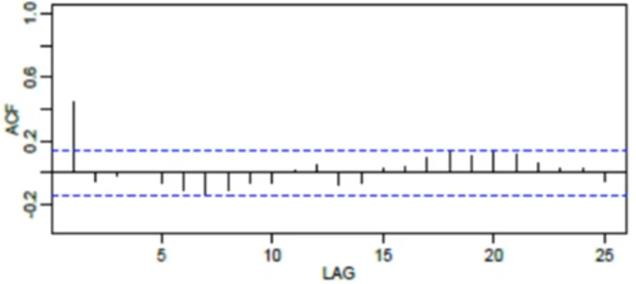
\includegraphics[width=0.85\textwidth]{images/u2_acf_pacf_example1.jpg}
    \caption{Sample ACF and PACF correlograms: Bars represent autocorrelation coefficients at each lag. Dashed horizontal lines are the significance bounds ($\pm 1.96/\sqrt{n}$). Bars extending beyond the bounds indicate statistically significant correlation at that lag. (Source: TSA course notes, ACF and PACF questions and rules)}
    \label{fig:u2_acf_pacf_1}
\end{figure}

\begin{figure}[H]
    \centering
    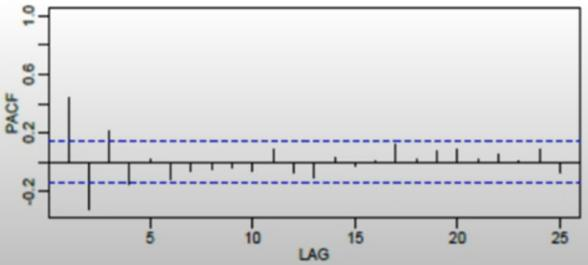
\includegraphics[width=0.85\textwidth]{images/u2_acf_pacf_example2.jpg}
    \caption{Correlogram examples showing different ACF/PACF patterns used for model identification. Comparing the decay pattern of ACF against the cutoff point of PACF determines whether the process is AR, MA, or ARMA. (Source: TSA course notes, ACF and PACF questions and rules)}
    \label{fig:u2_acf_pacf_2}
\end{figure}


\section{Unit 3: Linear Time Series Models}

\subsection{Motivation for Linear Time Series Models}

Studying linear time series models is highly motivating for several reasons. \textbf{Predictive Power}: Linear models provide a powerful framework for understanding and predicting future values. By studying these models, you gain insights into underlying patterns and trends, allowing accurate predictions in finance, economics, meteorology, and marketing. \textbf{Interpretability}: Linear models offer interpretability --- you can understand individual contributions of each variable and their impact on the time series, which is crucial for decision-making and policy planning. \textbf{Fundamental Understanding}: Studying linear models deepens understanding of autocorrelation, stationarity, and other fundamental properties, forming a solid foundation for advanced models like state-space models or neural networks. \textbf{Diagnostic Tools}: Linear models provide various diagnostic tools for assessing model adequacy --- evaluating performance, identifying outliers, checking residual autocorrelation, and testing model assumptions. \textbf{Practical Applications}: They are used for forecasting sales, predicting stock prices, analyzing economic trends, and understanding customer behavior. \textbf{Career Advancement}: Proficiency in time series modeling is highly sought after in finance, economics, data science, and operations research.

\subsection{The Autoregressive (AR) Model}

The autoregressive model of order $p$, denoted AR($p$), describes the relationship between an observation and its $p$ lagged values. The equation for an AR($p$) model is:
\[
X_t = c + \phi_1 X_{t-1} + \phi_2 X_{t-2} + \ldots + \phi_p X_{t-p} + \varepsilon_t
\]
where $c$ is a constant, $\phi_1, \ldots, \phi_p$ are the autoregressive parameters, and $\varepsilon_t$ is white noise with mean 0 and variance $\sigma^2$. For an AR($p$) process to be stationary, the roots of the characteristic equation $1 - \phi_1 z - \phi_2 z^2 - \ldots - \phi_p z^p = 0$ must lie \textbf{outside} the unit circle (i.e., $|z| > 1$).

\subsubsection{AR(1) Model}

The simplest and most studied case is AR(1):
\[
X_t = c + \phi_1 X_{t-1} + \varepsilon_t
\]
For stationarity, the parameter must satisfy $|\phi_1| < 1$. The mean is $\mu = \frac{c}{1 - \phi_1}$. The variance is $\gamma(0) = \frac{\sigma^2}{1 - \phi_1^2}$. The autocorrelation function is $\rho(h) = \phi_1^{|h|}$, which shows \textbf{exponential decay} (or damped oscillation if $\phi_1 < 0$). The PACF of an AR(1) process \textbf{cuts off sharply after lag 1}.

\begin{tcolorbox}[colback=blue!5!white,colframe=blue!75!black,title=\textbf{Worked Example 1: AR(1) Forecasting}]
\textbf{Given}: $X_t = 0.4 X_{t-1} + \varepsilon_t$, and current observation $X_t = 15$.

\textbf{Find}: One-step, two-step, and three-step ahead forecasts.

\textbf{Solution}:
\begin{enumerate}
    \item Stationarity check: $|\phi_1| = |0.4| = 0.4 < 1$. \textbf{Yes, stationary}.
    \item One-step forecast: $\hat{X}_{t+1|t} = 0.4 \times X_t = 0.4 \times 15 = 6.0$
    \item Two-step forecast: $\hat{X}_{t+2|t} = 0.4 \times \hat{X}_{t+1|t} = 0.4 \times 6.0 = 2.4$
    \item Three-step forecast: $\hat{X}_{t+3|t} = 0.4 \times 2.4 = 0.96$
\end{enumerate}
\textbf{Answer}: $\hat{X}_{t+1} = 6.0$, $\hat{X}_{t+2} = 2.4$, $\hat{X}_{t+3} = 0.96$.

\textbf{Interpretation}: As the forecast horizon increases, predictions converge toward the long-run mean ($\mu = 0$ for this zero-mean process). The geometric decay reflects the mean-reverting property of stationary AR processes. For an AR(1) with nonzero mean $c$, forecasts converge to $\mu = c/(1-\phi_1)$.
\end{tcolorbox}

\begin{tcolorbox}[colback=green!5!white,colframe=green!75!black,title=\textbf{Worked Example 2: AR(1) Unit Root Analysis}]
\textbf{Given}: Analyze the AR(1) process $X_t = \phi X_{t-1} + \varepsilon_t$ for $|\phi| < 1$, $|\phi| = 1$, and $|\phi| > 1$.

\textbf{Solution}:
\begin{itemize}
    \item \textbf{$|\phi| < 1$ (Stationary)}: Shocks die out geometrically. Mean = 0, variance = $\sigma^2/(1-\phi^2)$. The ACF decays exponentially: $\rho(h) = \phi^h$. The process is mean-reverting. This is the standard case for AR modeling.
    \item \textbf{$|\phi| = 1$ (Unit Root / Random Walk)}: Non-stationary. The series becomes $X_t = X_{t-1} + \varepsilon_t$. Variance grows as $t \cdot \sigma^2$ without bound. Shocks have permanent effects --- a shock at time $t$ affects all future values by exactly its magnitude. The ACF does not decay --- $\rho(h) \approx 1$ for all lags. Requires \textbf{first differencing}: $\Delta X_t = X_t - X_{t-1} = \varepsilon_t$, which is white noise and stationary.
    \item \textbf{$|\phi| > 1$ (Explosive)}: The series diverges exponentially. Each shock is amplified by $|\phi|$ in the next period. Mean does not exist (or is unstable); variance explodes even faster than the random walk. Such processes are rarely observed in economics but may appear in hyperinflation data. No standard time series model can handle this without transformation.
\end{itemize}
\end{tcolorbox}

\subsubsection{AR(2) Model}

The AR(2) model is:
\[
X_t = c + \phi_1 X_{t-1} + \phi_2 X_{t-2} + \varepsilon_t
\]
Stationarity requires that the roots of $1 - \phi_1 z - \phi_2 z^2 = 0$ lie outside the unit circle. Equivalently, the following conditions must hold:
\begin{itemize}
    \item $\phi_1 + \phi_2 < 1$
    \item $\phi_2 - \phi_1 < 1$
    \item $|\phi_2| < 1$
\end{itemize}
The ACF of AR(2) shows damped oscillation or exponential decay (depending on whether roots are complex or real), while the PACF cuts off sharply after lag 2. When the roots are complex conjugates, the ACF exhibits damped sinusoidal behavior --- this corresponds to pseudo-cyclical behavior in the time series.

\begin{tcolorbox}[colback=green!5!white,colframe=green!75!black,title=\textbf{Worked Example 3: AR(2) General Equation and Stationarity}]
\textbf{Given}: $X_t = 0.3 X_{t-1} + 0.4 X_{t-2} + \varepsilon_t$.

\textbf{Check}: Is this process stationary?

\textbf{Solution}:
\begin{enumerate}
    \item $\phi_1 = 0.3$, $\phi_2 = 0.4$
    \item Condition 1: $\phi_1 + \phi_2 = 0.3 + 0.4 = 0.7 < 1$ \checkmark
    \item Condition 2: $\phi_2 - \phi_1 = 0.4 - 0.3 = 0.1 < 1$ \checkmark
    \item Condition 3: $|\phi_2| = 0.4 < 1$ \checkmark
\end{enumerate}
\textbf{Answer}: \textbf{Stationary}. The characteristic equation $1 - 0.3z - 0.4z^2 = 0$ has roots $z = \frac{-0.3 \pm \sqrt{0.09 + 1.6}}{-0.8} = \frac{-0.3 \pm 1.30}{-0.8}$, giving $z_1 \approx -1.25$ and $z_2 \approx 2.0$. Both roots have magnitude greater than 1, confirming stationarity. The ACF will show exponential decay (real roots), and the PACF will cut off after lag 2.
\end{tcolorbox}

\subsection{The Moving Average (MA) Model}

The moving average model of order $q$, denoted MA($q$), describes the relationship between an observation and a linear combination of $q$ previous error terms (shocks):
\[
X_t = \mu + \varepsilon_t + \theta_1 \varepsilon_{t-1} + \theta_2 \varepsilon_{t-2} + \ldots + \theta_q \varepsilon_{t-q}
\]
MA models are \textbf{always stationary} because they are a finite sum of stationary white noise terms. However, they are only \textbf{invertible} if the roots of $\theta(z) = 1 + \theta_1 z + \ldots + \theta_q z^q = 0$ lie outside the unit circle. Invertibility ensures that the MA process can be represented as an infinite AR process.

\subsubsection{MA(1) Model}

\[
X_t = \mu + \varepsilon_t + \theta_1 \varepsilon_{t-1}
\]
The mean is $\mu$. The variance is $\gamma(0) = \sigma^2(1 + \theta_1^2)$. The autocovariance at lag 1 is $\gamma(1) = \theta_1 \sigma^2$, giving autocorrelation $\rho(1) = \frac{\theta_1}{1 + \theta_1^2}$. For $h > 1$, $\gamma(h) = 0$. The ACF of an MA(1) process \textbf{cuts off sharply after lag 1}. The PACF \textbf{tails off} gradually (damped exponential or oscillation).

\begin{tcolorbox}[colback=blue!5!white,colframe=blue!75!black,title=\textbf{Worked Example 4: MA(2) Autocorrelation and Identification}]
\textbf{Given}: $X_t = 15 + \varepsilon_t + 0.5\varepsilon_{t-1} - 0.2\varepsilon_{t-2}$.

\textbf{Find}: Identify the model. Compute $\rho_1$, $\rho_2$, and $\rho_3$.

\textbf{Solution}:
\begin{enumerate}
    \item Rewrite in standard form: $X_t = 15 + \varepsilon_t + 0.5\varepsilon_{t-1} - 0.2\varepsilon_{t-2}$.
    \item This is an \textbf{MA(2)} model with $\theta_1 = 0.5$, $\theta_2 = -0.2$, $\mu = 15$.
    \item Variance: $\gamma(0) = \sigma^2(1 + \theta_1^2 + \theta_2^2) = \sigma^2(1 + 0.25 + 0.04) = 1.29\sigma^2$
    \item Autocovariance lag 1: $\gamma(1) = \sigma^2(\theta_1 + \theta_1\theta_2) = \sigma^2(0.5 + (0.5)(-0.2)) = \sigma^2(0.5 - 0.1) = 0.4\sigma^2$
    \item Autocovariance lag 2: $\gamma(2) = \sigma^2 \theta_2 = -0.2\sigma^2$
    \item Autocovariance lag 3: $\gamma(3) = 0$
    \item Autocorrelations:
    \begin{itemize}
        \item $\rho_1 = \frac{\gamma(1)}{\gamma(0)} = \frac{0.4}{1.29} \approx 0.310$
        \item $\rho_2 = \frac{\gamma(2)}{\gamma(0)} = \frac{-0.2}{1.29} \approx -0.155$
        \item $\rho_3 = 0$
    \end{itemize}
\end{enumerate}
\textbf{Answer}: MA(2). $\rho_1 \approx 0.310$, $\rho_2 \approx -0.155$, $\rho_3 = 0$.

\textbf{Interpretation}: The ACF cuts off after lag 2, which is the signature of an MA(2) process. The positive $\rho_1$ indicates positive correlation between adjacent observations; the negative $\rho_2$ indicates a reversal pattern two periods apart.
\end{tcolorbox}

\begin{tcolorbox}[colback=green!5!white,colframe=green!75!black,title=\textbf{Worked Example 5: MA(2) Autocovariance}]
\textbf{Given}: $X_t = \varepsilon_t + 0.7\varepsilon_{t-1} + 0.3\varepsilon_{t-2}$.

\textbf{Find}: Autocovariance at lag 1 and lag 2.

\textbf{Solution}: $\theta_1 = 0.7$, $\theta_2 = 0.3$.
\begin{itemize}
    \item $\gamma(0) = \sigma^2(1 + 0.49 + 0.09) = 1.58\sigma^2$
    \item $\gamma(1) = \sigma^2(0.7 + 0.21) = 0.91\sigma^2$
    \item $\gamma(2) = \sigma^2 \times 0.3 = 0.3\sigma^2$
    \item $\gamma(h) = 0$ for $h > 2$
\end{itemize}
\textbf{Answer}: $\gamma(1) = 0.91\sigma^2$, $\gamma(2) = 0.3\sigma^2$.

\textbf{Interpretation}: The autocovariance decays to zero after lag 2. For MA($q$), only $q$ lags have non-zero autocovariance. This is why the ACF ``cutoff'' rule works for identifying MA order.
\end{tcolorbox}


\subsection{The ARMA Model}

The ARMA($p, q$) model combines autoregressive and moving average components:
\[
X_t = c + \sum_{i=1}^p \phi_i X_{t-i} + \varepsilon_t + \sum_{j=1}^q \theta_j \varepsilon_{t-j}
\]
ARMA models are more parsimonious than pure AR or pure MA models --- they can capture complex dynamics with fewer parameters. The benefits of ARMA include \textbf{Flexibility} --- capturing both short-term dependencies (via MA) and long-term dependencies (via AR); \textbf{Interpretability} --- coefficients provide insights into the relationship between current and past values; and \textbf{Forecasting} --- can forecast future values based on historical data. However, ARMA models assume stationarity, require correct model order selection (challenging, often using AIC/BIC), are sensitive to outliers, and have limited forecasting horizon due to error accumulation.

For an ARMA process: the ACF \textbf{tails off} gradually (decays exponentially or with damped sine waves), and the PACF \textbf{tails off} gradually. Neither cuts off sharply, which distinguishes ARMA from pure AR or pure MA. This dual tail-off pattern is the key identification signature.

\begin{figure}[H]
    \centering
    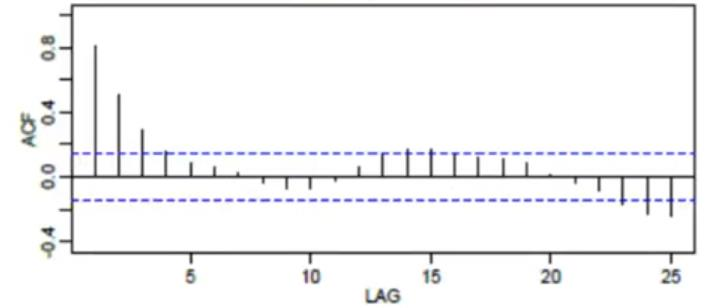
\includegraphics[width=0.85\textwidth]{images/u2_acf_pacf_example3.jpg}
    \caption{Correlogram patterns for AR($p$) model identification: PACF cuts off after lag $p$ while ACF tails off gradually (exponential decay or damped oscillation). The lag at which PACF becomes insignificant directly reveals the AR order. (Source: TSA course notes, ACF and PACF questions and rules)}
    \label{fig:u3_ar_identify}
\end{figure}

\begin{figure}[H]
    \centering
    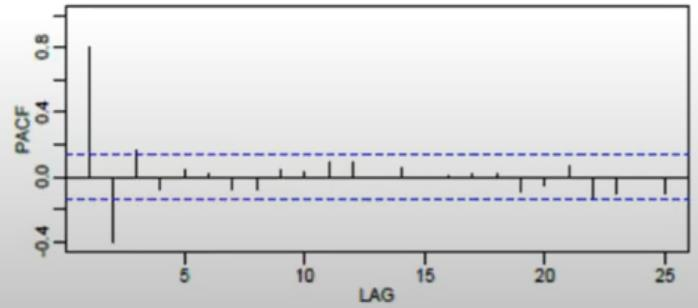
\includegraphics[width=0.85\textwidth]{images/u2_acf_pacf_example4.jpg}
    \caption{Correlogram patterns for MA($q$) model identification: ACF cuts off after lag $q$ while PACF tails off gradually. The lag at which ACF becomes insignificant directly reveals the MA order. (Source: TSA course notes, ACF and PACF questions and rules)}
    \label{fig:u3_ma_identify}
\end{figure}

\begin{figure}[H]
    \centering
    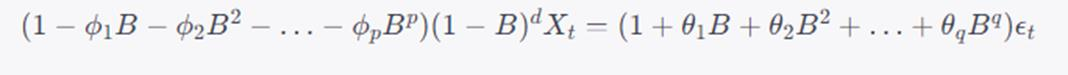
\includegraphics[width=0.85\textwidth]{images/u2_acf_pacf_example5.jpg}
    \caption{Correlogram showing ACF and PACF patterns for ARMA($p,q$) identification: Both ACF and PACF tail off gradually (no sharp cutoff), indicating a mixed ARMA process rather than pure AR or pure MA. (Source: TSA course notes, Module 2)}
    \label{fig:u3_arma_identify}
\end{figure}

\begin{figure}[H]
    \centering
    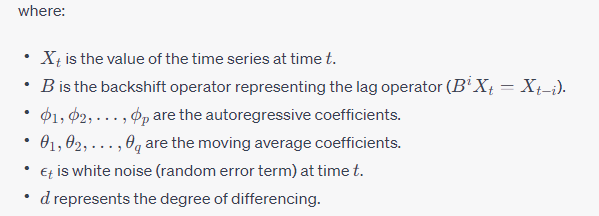
\includegraphics[width=0.85\textwidth]{images/u2_acf_pacf_example6.png}
    \caption{Correlogram summary: Comparison of ACF and PACF behaviours for AR, MA, and ARMA processes. AR($p$): PACF cutoff at lag $p$; MA($q$): ACF cutoff at lag $q$; ARMA($p,q$): both tail off; White noise: no significant spikes in either. (Source: TSA course notes, Module 2)}
    \label{fig:u3_summary}
\end{figure}

\begin{tcolorbox}[colback=blue!5!white,colframe=blue!75!black,title=\textbf{Worked Example 6: ARMA(1,1) Identification}]
\textbf{Given}: A time series shows gradual exponential decay in ACF and a significant spike at lag 1 in PACF with gradual decay afterward.

\textbf{Question}: Identify the model and justify.

\textbf{Solution}:
\begin{enumerate}
    \item ACF tails off gradually $\Rightarrow$ not pure MA (MA would cut off).
    \item PACF does not cut off sharply at a single lag $\Rightarrow$ not pure AR (AR would cut off).
    \item Both ACF and PACF tail off $\Rightarrow$ \textbf{ARMA} process.
    \item The single significant PACF spike at lag 1 suggests $p = 1$; the smooth ACF decay suggests $q = 1$.
    \item \textbf{Model}: ARMA(1,1): $X_t = c + \phi_1 X_{t-1} + \varepsilon_t + \theta_1 \varepsilon_{t-1}$
\end{enumerate}

\textbf{Interpretation}: When both ACF and PACF tail off, neither pure AR nor pure MA is adequate. The ARMA combination captures both autoregressive dependence (via $\phi_1$) and shock persistence (via $\theta_1$).
\end{tcolorbox}

\subsection{The ARIMA Model}

Many real-world time series are non-stationary due to trends or unit roots. The ARIMA($p, d, q$) model extends ARMA by adding \textbf{differencing} to achieve stationarity. The components are: \textbf{AR}($p$): autoregressive component of order $p$; \textbf{I}($d$): differencing of order $d$ to remove trends/unit roots; \textbf{MA}($q$): moving average component of order $q$. The general ARIMA($p, d, q$) equation for the differenced series is:
\[
\nabla^d X_t = c + \sum_{i=1}^p \phi_i \nabla^d X_{t-i} + \varepsilon_t + \sum_{j=1}^q \theta_j \varepsilon_{t-j}
\]
where $\nabla = (1 - B)$ is the difference operator and $B$ is the backshift operator. The benefits of ARIMA include flexibility in capturing trend and seasonality, reasonably accurate forecasts for stationary data, interpretable coefficients, and sound statistical theory for hypothesis testing and confidence intervals. Drawbacks include the stationarity requirement (which is addressed by differencing but may introduce information loss), limited handling of complex nonlinear patterns, challenging model selection for $p$, $d$, $q$, sensitivity to outliers, and computational intensity for large datasets.

\begin{tcolorbox}[colback=blue!5!white,colframe=blue!75!black,title=\textbf{Worked Example 7: ARIMA Parameter Interpretation}]
\textbf{Given}: Model (1,1,2). Identify and explain each parameter.

\textbf{Solution}:
\begin{itemize}
    \item $p=1$: One autoregressive term on the differenced series.
    \item $d=1$: First differencing applied to achieve stationarity (removes a stochastic trend / unit root).
    \item $q=2$: Two moving average terms on the differenced series.
    \item \textbf{Model equation}: $\nabla X_t = c + \phi_1 \nabla X_{t-1} + \varepsilon_t + \theta_1 \varepsilon_{t-1} + \theta_2 \varepsilon_{t-2}$
\end{itemize}

\textbf{Interpretation}: First differencing removes the unit root. The AR(1) component captures persistence in the differenced series, while the MA(2) component captures shock persistence over two periods.
\end{tcolorbox}

\begin{tcolorbox}[colback=green!5!white,colframe=green!75!black,title=\textbf{Worked Example 8: ACF/PACF Identification Cases}]
\textbf{Case A}: ACF cuts off after lag 1, PACF tails off gradually $\Rightarrow$ \textbf{MA(1)}. The ACF cutoff tells us the MA order directly.

\textbf{Case B}: ACF tails off exponentially, PACF cuts off after lag 2 $\Rightarrow$ \textbf{AR(2)}. The PACF cutoff tells us the AR order directly.

\textbf{Case C}: Both ACF and PACF tail off gradually $\Rightarrow$ \textbf{ARMA}. Neither pure AR nor pure MA. The orders must be determined by trial or information criteria.

\textbf{Case D}: Monthly data, ACF spikes at lag 12 with slow decay $\Rightarrow$ \textbf{SARIMA} with seasonal period $s=12$. The spike at the seasonal lag indicates seasonal structure.
\end{tcolorbox}

\subsection{The SARIMA Model}

For seasonal data, SARIMA($p,d,q$)($P,D,Q$)$_s$ extends ARIMA with seasonal components. The general equation using the backshift operator $B$ (where $B^k X_t = X_{t-k}$) is:
\[
\Phi_P(B^s)\phi_p(B)(1-B)^d(1-B^s)^D X_t = \Theta_Q(B^s)\theta_q(B)\varepsilon_t
\]
where $s$ is the seasonal period (e.g., 4 for quarterly, 12 for monthly), $\Phi_P(B^s)$ is the seasonal AR polynomial, $\Theta_Q(B^s)$ is the seasonal MA polynomial, $(1-B)^d$ is regular differencing, and $(1-B^s)^D$ is seasonal differencing. The parameters are: $p,d,q$ for the non-seasonal part; $P,D,Q$ for the seasonal part; and $s$ for the seasonal period.

SARIMA benefits include effective seasonal component handling, flexibility in modeling both non-seasonal and seasonal patterns, good forecasting accuracy for seasonal data, and interpretable parameters. Drawbacks include complexity in selecting seven parameters, computational intensity, limited handling of nonlinear patterns, and sensitivity to outliers.

\begin{tcolorbox}[colback=blue!5!white,colframe=blue!75!black,title=\textbf{Worked Example 9: SARIMA Model for Airline Data}]
\textbf{Given}: An airline company observes: (a) Trend, (b) Seasonality every 4 quarters, (c) Autoregressive structure.

\textbf{Find}: (a) General SARIMA equation, (b) Explain parameters, (c) Suggest suitable model, (d) Explain seasonal differencing.

\textbf{Solution}:
\begin{enumerate}
    \item General equation: $\Phi_P(B^4)\phi_p(B)(1-B)^d(1-B^4)^D X_t = \Theta_Q(B^4)\theta_q(B)\varepsilon_t$
    \item For quarterly data with trend and seasonality, typical choices: $d=1$ (remove trend), $D=1$ (remove seasonality), $p=1$ or 2 (AR structure), $q=1$ (MA structure), $P=1$, $Q=1$, $s=4$.
    \item \textbf{Suggested model}: SARIMA(1,1,1)(1,1,1)$_4$
    \item \textbf{Seasonal differencing}: $(1-B^4)X_t = X_t - X_{t-4}$ removes the seasonal component by subtracting the value from the same quarter one year ago. This is distinct from regular differencing $(1-B)X_t = X_t - X_{t-1}$ which removes the trend.
\end{enumerate}
\end{tcolorbox}

\subsection{Unit Roots, Integrated and Non-Invertible Processes}

\subsubsection{Unit Roots}

In linear time series analysis, a unit root is a property of a time series variable that indicates it is non-stationary. A unit root implies that the series has a root equal to 1 in its characteristic equation, meaning it has a stochastic trend. The series has a tendency to wander but does not converge to a fixed value. Unit roots are associated with persistent shocks or random fluctuations. The presence of unit roots poses challenges because it violates the stationarity assumptions of many statistical techniques. The most common remedy is differencing: taking the difference between consecutive observations removes the trend and often makes the series stationary. If differencing once leads to stationarity, the series is said to be \textbf{integrated of order one}, denoted I(1). If further differencing is required, it is I(2), and so on.

\subsubsection{Integrated Processes}

An integrated process of order $d$, denoted I($d$), can be represented as:
\[
(1 - B)^d Y_t = X_t
\]
where $Y_t$ is the original non-stationary time series, $X_t$ is the differenced (stationary) series, $B$ is the backshift operator, and $d$ is the order of differencing. When $(1-B)^d$ is applied to $Y_t$, it transforms the non-stationary series into a stationary series $X_t$.

\subsubsection{Non-Invertible Processes}

A non-invertible process refers to a situation where it is not possible to recover the original series from its differenced version. The differenced series does not contain enough information to reconstruct the original series accurately. This may arise when multiple differencing steps are applied or if the original series has a stochastic trend that cannot be fully removed through differencing. For MA processes, non-invertibility occurs when roots of the MA polynomial lie inside the unit circle, meaning the MA representation is not unique and cannot be written as a convergent infinite AR process.

\subsection{Box-Jenkins Model Selection}

The Box-Jenkins methodology is an iterative and exploratory approach for selecting ARIMA models. It involves three main stages: \textbf{Identification}: examining the time series plot, ACF, and PACF to determine appropriate values of $p$, $d$, and $q$. Non-stationarity is detected by slowly decaying ACF, and differencing is applied until stationarity is achieved. \textbf{Estimation}: estimating parameters of the selected model using maximum likelihood or least squares. \textbf{Diagnostic Checking}: examining residuals for whiteness (Ljung-Box test), normality, and constant variance. If residuals show patterns, the model is inadequate and must be revised. Model selection criteria such as AIC and BIC are used to compare candidate models and penalize excessive parameters.

\begin{tcolorbox}[colback=green!5!white,colframe=green!75!black,title=\textbf{Worked Example 10: ACF/PACF Model Identification}]
\textbf{Given}: A time series shows gradual exponential decay in ACF and sharp cutoff at lag 2 in PACF.

\textbf{Identify}: The model, write its equation, and justify theoretically.

\textbf{Solution}:
\begin{enumerate}
    \item PACF cuts off sharply after lag 2 $\Rightarrow$ AR order $p = 2$.
    \item ACF tails off gradually (exponential decay) $\Rightarrow$ consistent with AR(2).
    \item \textbf{Model}: AR(2): $X_t = c + \phi_1 X_{t-1} + \phi_2 X_{t-2} + \varepsilon_t$
    \item Theoretical justification: For an AR($p$) process, the PACF cuts off after lag $p$ because the direct relationship between $X_t$ and $X_{t-p}$ is fully captured by the AR coefficients, and no additional direct relationship exists at higher lags. The ACF tails off because the AR structure creates indirect correlations at all lags through the chain of autoregressive dependencies.
\end{enumerate}
\end{tcolorbox}

\subsection{Simulating from an Autoregressive Process}

To simulate from an autoregressive process, follow these steps. First, define the order $p$ and specify the AR coefficients $\phi_1, \ldots, \phi_p$. Generate a sequence of random noise $\varepsilon_t$ from a standard normal distribution (mean 0, variance 1). Choose initial values $X_1, \ldots, X_p$. Then iterate: for each time step $t > p$, compute $X_t = \phi_1 X_{t-1} + \ldots + \phi_p X_{t-p} + \varepsilon_t$. Repeat for the desired number of observations. The stationarity of the simulated series depends on the AR coefficients --- if $|\phi_1| < 1$ for AR(1), or if all characteristic roots lie outside the unit circle for higher orders, the simulated series will be stationary.


\section{Unit 4: Prediction and Forecasting}

\subsection{Using Prediction in Estimating Time Series}

A systematic approach to time series forecasting involves several stages. First, \textbf{define the problem}: identify the variable to forecast and the forecast horizon (next week, month, or year). Second, \textbf{data collection and exploration}: gather historical data and visualize patterns, seasonality, and trends using time plots and autocorrelation plots. Third, \textbf{data preprocessing}: handle missing values, outliers, and transform the data to make it stationary through differencing or log transformations. Fourth, \textbf{train-test split}: reserve recent data for evaluation. Fifth, \textbf{feature engineering}: extract lag values, rolling averages, seasonal dummies, and other domain-specific features. Sixth, \textbf{choose a model}: ARIMA, SARIMA, machine learning models, or deep learning (LSTM/GRU). Seventh, \textbf{model training}: estimate parameters and tune hyperparameters. Eighth, \textbf{model evaluation}: use MAE, MSE, RMSE on the test set. Ninth, \textbf{fine-tuning}: adjust based on residual diagnostics. Tenth, \textbf{prediction and monitoring}: deploy and monitor performance over time, incorporating external factors if needed.

\subsection{Forecasting for Autoregressive Processes}

For an AR($p$) process, the optimal $h$-step ahead forecast is computed recursively using the estimated model. The one-step ahead forecast is $\hat{X}_{t+1|t} = c + \phi_1 X_t + \ldots + \phi_p X_{t-p+1}$. For multi-step forecasts, future observed values are replaced by their forecasts: $\hat{X}_{t+h|t} = c + \phi_1 \hat{X}_{t+h-1|t} + \ldots + \phi_p \hat{X}_{t+h-p|t}$, where for $h \leq p$, some values on the right are actual observations and some are forecasts. As $h \to \infty$, the forecast converges to the unconditional mean $\mu = c/(1 - \phi_1 - \ldots - \phi_p)$ for stationary processes.

\subsection{Forecasting for ARMA Processes}

For ARMA($p,q$), forecasting is more involved because future error terms $\varepsilon_{t+h}$ are unknown. For $h \leq q$, the forecast uses the estimated residuals; for $h > q$, future errors are set to their expected value of zero. The forecast is computed recursively by substituting observed values (or their forecasts) for past $X$ and estimated residuals (or zero) for past $\varepsilon$. Prediction intervals are computed from the forecast error variance, which depends on the MA coefficients and grows with the horizon.

\subsection{Forecasting Using the Infinite Past}

Forecasting a time series using an ``infinite past'' refers to using all available historical data to make predictions. In practice, we are limited by finite data, but for stationary processes with exponentially decaying dependence, the influence of very old observations becomes negligible. For an AR(1) process, the optimal linear predictor based on the infinite past is $\hat{X}_{t+1} = \phi_1 X_t$, and the influence of $X_{t-k}$ decays as $\phi_1^k$. The prediction error variance converges to the unconditional variance $\sigma^2/(1-\phi_1^2)$ for one-step forecasts and grows for multi-step forecasts.

\subsection{Levinson-Durbin Algorithm}

The Levinson-Durbin algorithm is a recursive method for estimating autoregressive coefficients and predicting future values based on a finite past. It is computationally efficient, requiring $O(p^2)$ operations rather than $O(p^3)$ for direct matrix inversion. The algorithm proceeds as follows: \textbf{Initialization}: set the first reflection coefficient $k_1 = \rho(1)$ and the first AR coefficient $a_{1,1} = k_1$, with prediction error variance $P_1 = \gamma(0)(1 - k_1^2)$. \textbf{Iteration}: for $m = 2, 3, \ldots, p$, compute the reflection coefficient $k_m$ using the Durbin formula:
\[
k_m = \frac{\rho(m) - \sum_{j=1}^{m-1} a_{m-1,j} \rho(m-j)}{1 - \sum_{j=1}^{m-1} a_{m-1,j} \rho(j)}
\]
Then update the AR coefficients: $a_{m,m} = k_m$ and $a_{m,j} = a_{m-1,j} - k_m a_{m-1,m-j}$ for $j = 1, \ldots, m-1$. Update the prediction error variance: $P_m = P_{m-1}(1 - k_m^2)$. \textbf{Output}: the final AR coefficients $a_{p,1}, \ldots, a_{p,p}$ and the prediction error variance $P_p$.

The Levinson-Durbin algorithm is particularly useful in real-time applications such as speech and audio processing, where fast recursive updates of predictors are essential.

\subsection{The Kalman Filter}

The Kalman filter is a mathematical algorithm for estimating the state of a linear dynamic system from noisy measurements. In time series analysis, it is useful for tracking and predicting the evolution of a system even when measurements are subject to noise. The Kalman filter operates in two stages: \textbf{Prediction}: predict the next state $\hat{x}_{t|t-1}$ and its covariance $P_{t|t-1}$ based on the system dynamics $x_t = F x_{t-1} + w_t$ (where $w_t$ is process noise). \textbf{Update}: obtain a measurement $z_t = H x_t + v_t$ (where $v_t$ is measurement noise), compute the Kalman gain $K_t = P_{t|t-1} H^T (H P_{t|t-1} H^T + R)^{-1}$, update the state estimate $\hat{x}_{t|t} = \hat{x}_{t|t-1} + K_t (z_t - H \hat{x}_{t|t-1})$, and update the covariance $P_{t|t} = (I - K_t H) P_{t|t-1}$. The Kalman gain determines how much weight to give to the new measurement versus the prediction. Variants include the Extended Kalman Filter (EKF) for mildly nonlinear systems and the Unscented Kalman Filter (UKF) for strongly nonlinear systems.

\subsection{Automated Forecasting Systems}

\subsubsection{Auto-ARIMA}

Auto-ARIMA automates the Box-Jenkins model selection process. It performs: automatic differencing (ADF or KPSS test to determine $d$), grid search over $p$ and $q$ within specified ranges, and model selection using AIC/BIC. The algorithm iteratively tests differencing orders, fits ARMA models, and selects the best combination. Popular implementations include the `pmdarima` library in Python and `auto.arima` in R.

\subsubsection{Prophet}

Prophet, developed by Facebook (Meta), is designed for forecasting daily observations with strong seasonality and holiday effects. It models the time series as $y(t) = g(t) + s(t) + h(t) + \varepsilon_t$, where $g(t)$ is the trend (piecewise linear or logistic), $s(t)$ is the seasonal component (Fourier series), and $h(t)$ is the holiday effect. Prophet is robust to missing data, outliers, and shifts in trend, and requires minimal tuning.

\subsubsection{AutoML for Time Series}

AutoML systems automate the entire pipeline: preprocessing (missing value imputation, outlier detection, stationarity testing), feature engineering (lag features, rolling statistics, date features), model selection (ARIMA, ETS, Prophet, XGBoost, neural networks), hyperparameter optimization (Bayesian optimization, random search), and ensemble methods (stacking, blending). Integration with hashing techniques allows efficient feature storage and retrieval for high-frequency time series.

\begin{tcolorbox}[colback=blue!5!white,colframe=blue!75!black,title=\textbf{Worked Example 11: Least Squares Trend Fitting}]
\textbf{Given}: Annual production (thousand units): Year 2016=45, 2017=52, 2018=50, 2019=60, 2020=63.

\textbf{Find}: (a) Straight-line trend using Least Squares, (b) Trend values, (c) Forecast for 2021, (d) Interpret the slope.

\textbf{Solution}: Let $t = -2, -1, 0, 1, 2$ (centered coding for computational convenience).
\begin{itemize}
    \item $\sum t = 0$, $\sum Y = 45+52+50+60+63 = 270$, $n=5$
    \item $\sum t^2 = 4+1+0+1+4 = 10$
    \item $\sum tY = (-2)(45)+(-1)(52)+0(50)+1(60)+2(63) = -90-52+0+60+126 = 44$
    \item Slope: $b = \frac{n\sum tY - \sum t \sum Y}{n\sum t^2 - (\sum t)^2} = \frac{5(44) - 0}{5(10) - 0} = \frac{220}{50} = 4.4$
    \item Intercept: $a = \bar{Y} - b\bar{t} = 270/5 - 4.4(0) = 54$
    \item Trend: $\hat{Y}_t = 54 + 4.4t$
\end{itemize}
Trend values: 2016 ($t=-2$): 45.2; 2017: 49.6; 2018: 54.0; 2019: 58.4; 2020: 62.8.

Forecast 2021 ($t=3$): $\hat{Y}_{2021} = 54 + 4.4(3) = 54 + 13.2 = 67.2$ thousand units.

\textbf{Slope interpretation}: Output increases by approximately 4.4 thousand units per year on average.
\end{tcolorbox}


\section{Unit 5: Models with Trend, Unit Root Tests, and Monte Carlo}

\subsection{Removing Trend}

Non-stationary time series often contain trends that must be removed before applying standard models. Common detrending techniques include: \textbf{Differencing}: computing $\Delta X_t = X_t - X_{t-1}$ removes a linear stochastic trend (unit root). Higher-order differencing removes polynomial trends. \textbf{Regression Detrending}: fitting a deterministic trend model (linear, polynomial, or exponential) and subtracting the fitted values yields a stationary residual series. \textbf{Hodrick-Prescott Filter}: decomposes a series into trend and cyclical components by minimizing a penalized sum of squared deviations. \textbf{Moving Average Smoothing}: a centered moving average removes short-term fluctuations, revealing the underlying trend.

\subsection{Dickey-Fuller Tests}

The Dickey-Fuller test tests the null hypothesis that a unit root is present in an autoregressive model. The basic DF test for AR(1) with no drift regresses $\Delta X_t$ on $X_{t-1}$ and tests whether the coefficient $\gamma = 0$ in:
\[
\Delta X_t = \gamma X_{t-1} + \varepsilon_t
\]
Under the null, $\gamma = 0$ (unit root). Under the alternative, $\gamma < 0$ (stationary). The test statistic does not follow the standard t-distribution --- critical values are derived from Dickey-Fuller distributions via simulation. The \textbf{Augmented Dickey-Fuller (ADF) Test} extends this by adding lagged differences of $X_t$ to control for higher-order autocorrelation:
\[
\Delta X_t = \gamma X_{t-1} + \sum_{i=1}^p \delta_i \Delta X_{t-i} + \varepsilon_t
\]
Three specifications exist: (1) no constant, no trend; (2) with constant (drift); (3) with constant and trend. The ADF critical values depend on the specification. The \textbf{Phillips-Perron (PP) Test} is a non-parametric alternative that does not require choosing lag length --- it adjusts the DF test statistic for serial correlation and heteroskedasticity using Newey-West standard errors.

\begin{tcolorbox}[colback=blue!5!white,colframe=blue!75!black,title=\textbf{Worked Example 12: ADF Test Interpretation}]
\textbf{Case A}: Test Statistic = 0.815, p-value = 0.9919, Critical Values: 1\%=-3.482, 5\%=-2.884, 10\%=-2.579.

\textbf{Decision}: The test statistic (0.815) is \textbf{greater} than all critical values (less negative). p-value (0.9919) >> 0.05. \textbf{Fail to reject null hypothesis of unit root}. The series is \textbf{non-stationary}.

\textbf{Case B}: Test Statistic = -4.4448, p-value = 0.000247, Critical Values: 1\%=-3.482, 5\%=-2.884, 10\%=-2.579.

\textbf{Decision}: The test statistic (-4.4448) is \textbf{more negative} than all critical values. p-value (0.000247) << 0.05. \textbf{Reject null hypothesis}. The series is \textbf{stationary} (no unit root).
\end{tcolorbox}

\subsection{The Monte Carlo Method}

Monte Carlo simulation generates multiple random paths of a time series using estimated model parameters to assess uncertainty, risk, and model behavior. Applications include: \textbf{Stochastic Time Series Generation}: creating synthetic data mimicking observed statistical properties for testing models; \textbf{Forecasting}: generating multiple future scenarios to estimate prediction distributions and intervals; \textbf{Risk Assessment}: estimating probability distributions of financial outcomes; and \textbf{Scenario Analysis}: exploring impact of policy changes or events.

The process involves: (1) collecting historical data; (2) choosing a model (ARIMA, GARCH, etc.); (3) estimating parameters; (4) generating multiple random paths using the model and random innovations; (5) varying key assumptions across simulations; and (6) analyzing the distribution of outcomes.

\begin{tcolorbox}[colback=blue!5!white,colframe=blue!75!black,title=\textbf{Worked Example 13: Monte Carlo for ADF Critical Values}]
\textbf{Problem}: A researcher tests for a unit root using ADF. The test statistic distribution is unknown for their specific sample size and model specification. How can Monte Carlo generate critical values?

\textbf{Solution}:
\begin{enumerate}
    \item Assume the null hypothesis of a unit root: $X_t = X_{t-1} + \varepsilon_t$ with $\varepsilon_t \sim N(0,1)$.
    \item Generate $N$ (e.g., 10,000) simulated series of length $T$ under the null.
    \item For each simulated series, compute the ADF test statistic with the same specification (constant, trend, lag length).
    \item The empirical distribution of these $N$ statistics gives Monte Carlo critical values.
    \item For 5\% significance, take the 5th percentile of the simulated statistics.
    \item Compare the observed test statistic to these critical values for inference.
\end{enumerate}
\textbf{Advantage}: Does not rely on asymptotic approximations; works for any sample size or model variant. This is particularly useful when standard critical value tables do not cover the exact sample size or model specification.
\end{tcolorbox}


\section{Unit 6: Multiequation Time Series Models}

\subsection{Intervention Analysis}

Intervention analysis assesses the effect of a known event on a time series. The general approach models the series as an ARIMA process plus an intervention component: $Y_t = \text{ARIMA} + \omega I_t + \varepsilon_t$. Common intervention types include: \textbf{Step intervention}: $I_t = 0$ for $t < T$, $I_t = 1$ for $t \geq T$, producing a permanent level shift. \textbf{Pulse intervention}: $I_t = 1$ at $t = T$ and 0 otherwise, producing a temporary shock. \textbf{Ramp intervention}: linear increase starting at $T$. The parameter $\omega$ measures the magnitude of the intervention effect, and its significance is tested using standard t-tests.

\begin{tcolorbox}[colback=blue!5!white,colframe=blue!75!black,title=\textbf{Worked Example 14: Intervention Analysis -- Speed Limit}]
\textbf{Problem}: North Carolina highway fatality rates, monthly $n=86$. At month 71, speed limit lowered from 70 to 55 mph. Determine the intervention effect.

\textbf{Solution}:
\begin{enumerate}
    \item Model the pre-intervention period (months 1--70) with ARIMA to establish a baseline.
    \item Introduce a step intervention variable: $I_t = 0$ for $t < 71$, $I_t = 1$ for $t \geq 71$.
    \item Fit the full model: $Y_t = \text{ARIMA}(p,d,q) + \omega I_t + \varepsilon_t$.
    \item Estimate $\omega$: the change in mean fatality rate attributable to the policy.
    \item If $\omega < 0$ and statistically significant ($p < 0.05$), conclude the speed limit reduction decreased fatalities.
\end{enumerate}
\textbf{Interpretation}: A negative and significant $\omega$ provides evidence that the intervention had the intended effect. The ARIMA component accounts for autocorrelation in the fatality rate series, ensuring that the intervention effect is not confounded with natural temporal patterns.
\end{tcolorbox}

\subsection{Autoregressive Distributed Lag (ADL) Model}

The ADL model analyzes long-run relationships and short-run dynamics between a dependent variable $Y_t$ and independent variables $X_t$:
\[
Y_t = \alpha_0 + \sum_{i=1}^p \alpha_i Y_{t-i} + \sum_{j=0}^q \beta_j X_{t-j} + \varepsilon_t
\]
The AR component captures the short-term dynamics of $Y_t$ via its own lags. The distributed lag component captures lagged effects of $X_t$ on $Y_t$. ADL models are used when cointegration (long-run equilibrium) is suspected --- even if variables exhibit short-term fluctuations, they tend to move together in the long run. ARDL models are particularly useful for non-stationary data and can be used for policy analysis, forecasting, and studying the impact of economic shocks.

\subsection{Transfer Function Model}

The transfer function model describes how an input series $X_t$ affects an output series $Y_t$:
\[
Y_t = H(B) X_t + E_t
\]
where $H(B)$ is the transfer function expressed in terms of the backshift operator $B$, and $E_t$ is the error term (often modeled as an ARMA process). The transfer function captures dynamic causal relationships between variables, accounting for time lags and different weighting of past values of $X$ on $Y$. It is estimated using prewhitening: first fit an ARMA model to $X_t$ to obtain white noise residuals, then cross-correlate these residuals with $Y_t$ to identify the transfer function structure.

\begin{tcolorbox}[colback=green!5!white,colframe=green!75!black,title=\textbf{Worked Example 15: ADL(2,2) Transfer Function Derivation}]
For $p=2$ and $q=2$, the ADL model is:
\[
Y_t = \alpha_0 + \alpha_1 Y_{t-1} + \alpha_2 Y_{t-2} + \beta_0 X_t + \beta_1 X_{t-1} + \beta_2 X_{t-2} + \varepsilon_t
\]
In transfer function form, rewrite using the backshift operator $B$:
\[
(1 - \alpha_1 B - \alpha_2 B^2) Y_t = \alpha_0 + (\beta_0 + \beta_1 B + \beta_2 B^2) X_t + \varepsilon_t
\]
\[
Y_t = \frac{\alpha_0}{1 - \alpha_1 B - \alpha_2 B^2} + \frac{\beta_0 + \beta_1 B + \beta_2 B^2}{1 - \alpha_1 B - \alpha_2 B^2} X_t + \frac{1}{1 - \alpha_1 B - \alpha_2 B^2} \varepsilon_t
\]
The rational polynomial $H(B) = \frac{\beta_0 + \beta_1 B + \beta_2 B^2}{1 - \alpha_1 B - \alpha_2 B^2}$ is the transfer function. Its impulse response --- the coefficients when $H(B)$ is expanded as a power series in $B$ --- shows how a one-unit shock in $X$ propagates through $Y$ over time. For example, if $\alpha_1 = 0.5$, $\alpha_2 = 0$, $\beta_0 = 1$, $\beta_1 = 0.3$, then $H(B) = (1 + 0.3B)/(1 - 0.5B) = 1 + 0.8B + 0.4B^2 + 0.2B^3 + \ldots$, showing a decaying response pattern.
\end{tcolorbox}

\subsection{Vector Autoregressive (VAR) Model}

A VAR model captures interdependencies between multiple time series. A VAR($p$) for $k$ variables is:
\[
\mathbf{Y}_t = \mathbf{c} + \sum_{i=1}^p \mathbf{A}_i \mathbf{Y}_{t-i} + \boldsymbol{\varepsilon}_t
\]
where $\mathbf{Y}_t$ is a $k \times 1$ vector, $\mathbf{A}_i$ are $k \times k$ coefficient matrices, and $\boldsymbol{\varepsilon}_t$ is a vector of white noise innovations (often with contemporaneous covariance $\mathbf{\Sigma}$). VAR models are useful for understanding dynamic relationships among variables, Granger causality testing, forecasting multiple related series jointly, and policy analysis via impulse response functions.

\begin{tcolorbox}[colback=blue!5!white,colframe=blue!75!black,title=\textbf{Worked Example 16: VAR for Stock Prices and Exchange Rates}]
\textbf{Problem}: Two series --- stock prices ($S_t$) and exchange rates ($E_t$). Apply VAR to analyze interdependence.

\textbf{Solution}: A VAR(1) model:
\[
\begin{pmatrix} S_t \\ E_t \end{pmatrix} = \begin{pmatrix} c_1 \\ c_2 \end{pmatrix} + \begin{pmatrix} a_{11} & a_{12} \\ a_{21} & a_{22} \end{pmatrix} \begin{pmatrix} S_{t-1} \\ E_{t-1} \end{pmatrix} + \begin{pmatrix} \varepsilon_{1t} \\ \varepsilon_{2t} \end{pmatrix}
\]
\begin{itemize}
    \item $a_{12}$: Effect of past exchange rate on current stock price.
    \item $a_{21}$: Effect of past stock price on current exchange rate.
    \item If $a_{12}$ is significant, exchange rates Granger-cause stock prices.
    \item Impulse response: Trace how a shock to $E_t$ propagates to $S_{t+h}$ over $h=1,2,\ldots$
\end{itemize}
\textbf{Granger causality test}: Regress $S_t$ on its own lags and lags of $E_t$. If the coefficients on $E_t$ lags are jointly significant (F-test), $E$ Granger-causes $S$.
\end{tcolorbox}

\subsection{Vector Error Correction Model (VECM)}

When non-stationary variables are cointegrated (share a long-run equilibrium relationship), the VAR in levels is misspecified due to the unit roots. The VECM reparameterizes the VAR in differences to include an error correction term:
\[
\Delta \mathbf{Y}_t = \mathbf{\alpha} \mathbf{\beta}^T \mathbf{Y}_{t-1} + \sum_{i=1}^{p-1} \mathbf{\Gamma}_i \Delta \mathbf{Y}_{t-i} + \boldsymbol{\varepsilon}_t
\]
where $\mathbf{\alpha} \mathbf{\beta}^T \mathbf{Y}_{t-1}$ is the error correction term. $\mathbf{\beta}$ contains the cointegrating vectors (long-run equilibrium relationships), and $\mathbf{\alpha}$ contains the adjustment speeds (how quickly each variable returns to equilibrium). The rank of $\mathbf{\alpha} \mathbf{\beta}^T$ determines the number of cointegrating relationships.

\subsection{Structural VAR (SVAR)}

Standard VAR treats all variables symmetrically and does not identify structural shocks. The SVAR imposes restrictions based on economic theory to identify structural (as opposed to reduced-form) innovations. The structural form is $\mathbf{B} \mathbf{Y}_t = \mathbf{\Gamma}_0 + \sum \mathbf{\Gamma}_i \mathbf{Y}_{t-i} + \mathbf{u}_t$, where $\mathbf{u}_t$ are uncorrelated structural shocks. Identification requires $k(k-1)/2$ restrictions on $\mathbf{B}$ or the contemporaneous covariance matrix. Common identification schemes include recursive (Cholesky) ordering, short-run restrictions, and long-run restrictions (Blanchard-Quah).

\subsection{Time-Varying Parameter VAR (TVP-VAR)}

Standard VAR assumes constant coefficients, which may fail during structural breaks (e.g., financial crises). TVP-VAR allows parameters to evolve over time:
\[
\mathbf{Y}_t = \mathbf{c}_t + \sum_{i=1}^p \mathbf{A}_{i,t} \mathbf{Y}_{t-i} + \boldsymbol{\varepsilon}_t
\]
Coefficients typically follow random walks: $\mathbf{A}_{i,t} = \mathbf{A}_{i,t-1} + \mathbf{v}_{i,t}$. This captures changing relationships between variables, such as GDP growth and inflation, before and after a financial crisis. TVP-VAR is estimated using Kalman filtering or MCMC methods.

\subsection{Bayesian VAR (BVAR)}

When the number of variables is large relative to observations, OLS estimates become unstable due to the ``curse of dimensionality.'' BVAR applies shrinkage priors to regularize coefficients. The Minnesota prior is the most common: own lags are centered at 1 (random walk), cross-lags are centered at 0, and the tightness hyperparameter controls the strength of shrinkage. The posterior combines prior beliefs with data evidence, yielding stable estimates even with many variables. BVAR improves out-of-sample forecasts compared to unrestricted VAR.

\begin{tcolorbox}[colback=green!5!white,colframe=green!75!black,title=\textbf{Worked Example 17: BVAR for Energy Demand}]
\textbf{Problem}: Energy demand depends on temperature, industrial output, and population. Standard VAR becomes too complex and unstable with 4 variables and limited data.

\textbf{Solution}: Use BVAR with Minnesota prior:
\begin{itemize}
    \item Prior for own lags (e.g., demand on lagged demand): centered at 1 with moderate variance.
    \item Prior for cross-lags (e.g., demand on temperature): centered at 0 with small variance (strong shrinkage toward 0).
    \item Tightness hyperparameter $\lambda$: controls overall shrinkage. Smaller $\lambda$ = stronger shrinkage.
    \item Posterior = Prior + Likelihood. With limited data, the prior dominates for cross-lags, stabilizing estimates.
\end{itemize}
\textbf{Result}: Improved out-of-sample forecasts and interpretable coefficient patterns compared to unrestricted VAR.
\end{tcolorbox}


\section{Unit 7: Multivariate Time Series}

\subsection{Background: Sequences and Functions}

A time series is essentially a sequence of data points collected over time, denoted $\{Y_t\}$ for time index $t$. These sequences can be univariate (one variable) or multivariate (multiple variables observed simultaneously) and can have various frequencies (hourly, daily, weekly, monthly). Analyzing underlying patterns and trends --- seasonality, cycles, and irregular components --- is the key aspect of time series analysis.

Functions in time series analysis represent and model relationships within the data. The \textbf{trend function} models the long-term direction of the time series. The \textbf{seasonal function} captures repetitive patterns at fixed intervals. The \textbf{autocorrelation function (ACF)} and \textbf{partial autocorrelation function (PACF)} identify and quantify the relationship between current and past observations --- ACF measures correlation at different lags, while PACF identifies the direct effect of past observations excluding intermediate lags.

\subsection{Convolution}

Convolution is a mathematical operation used for filtering, smoothing, and feature extraction in time series analysis. \textbf{Moving Averages}: convolution implements moving averages by convolving the time series with a kernel of equally weighted coefficients over a sliding window. \textbf{Convolutional Neural Networks (CNNs)}: 1D convolutional layers slide a small window over the time series and perform convolution to extract local patterns and features. \textbf{Cross-Correlation}: a variation of convolution used to measure similarity between two time series or detect relationships between them, useful for finding similarities in financial time series or aligning two series for analysis.

Mathematically, the discrete convolution of sequences $x$ and $h$ is $(x * h)_t = \sum_{k=-\infty}^{\infty} x_k h_{t-k}$. For a moving average filter of length $m$, the kernel $h_k = 1/m$ for $k = 0, \ldots, m-1$, and the convolution produces the smoothed series.

\subsection{Spectral Representations and Mean Squared Error}

\subsubsection{Spectral Representations}

Spectral representations decompose time series data in the frequency domain, revealing underlying periodic components. The \textbf{Fourier Transform} transforms a time-domain signal into its frequency-domain representation, decomposing a time series into sinusoidal components with associated frequencies, phases, and magnitudes. This provides insights into periodic patterns and dominant frequencies. The \textbf{Power Spectral Density (PSD)} quantifies how the variance of a time series is distributed across different frequencies. It is particularly useful for identifying dominant frequencies, understanding periodicity, and detecting seasonality. Spectral representations are essential in signal processing, control systems, and physics for understanding frequency characteristics.

\subsubsection{Mean Squared Error}

Mean Squared Error (MSE) is a widely used metric for evaluating forecasting model accuracy:
\[
\text{MSE} = \frac{1}{n} \sum_{t=1}^n (y_t - \hat{y}_t)^2
\]
Lower MSE indicates better predictive performance. MSE is sensitive to outliers (giving more weight to larger errors), so alternatives like Mean Absolute Error (MAE) or Root Mean Squared Error (RMSE) may be preferred. MSE is valuable for comparing different forecasting models and selecting the one with the smallest error.

\subsection{Multivariate Time Series Regression: Conditional Independence}

Conditional independence is essential for understanding relationships between variables in multivariate time series. It implies that two variables are conditionally independent if, after conditioning on other relevant variables, there is no direct causal relationship between them. The \textbf{Granger Causality Test} assesses conditional independence and causality: it tests whether past values of one variable significantly improve the prediction of another variable beyond the information provided by its own past values and other predictors. Without considering conditional independence, multivariate analysis can lead to \textbf{spurious correlations} --- cases where two variables appear related but the relationship is actually caused by a common third variable. Model specification must correctly account for conditional independence to avoid misleading results.

\subsection{Partial Correlation and Coherency}

\textbf{Partial correlation} measures the correlation between two time series after removing the linear effect of one or more additional variables. It quantifies the direct relationship between two variables, controlling for confounding factors. For three variables $X$, $Y$, and $Z$, the partial correlation between $X$ and $Y$ controlling for $Z$ is:
\[
\rho_{XY.Z} = \frac{\rho_{XY} - \rho_{XZ}\rho_{YZ}}{\sqrt{(1-\rho_{XZ}^2)(1-\rho_{YZ}^2)}}
\]

\textbf{Coherency} (or magnitude squared coherence) in the frequency domain measures the correlation between two time series at each frequency. It is computed from the cross-spectral density and the individual power spectral densities:
\[
C_{xy}(f) = \frac{|S_{xy}(f)|^2}{S_{xx}(f) S_{yy}(f)}
\]
where $S_{xy}(f)$ is the cross-spectral density and $S_{xx}(f)$, $S_{yy}(f)$ are the power spectral densities. Coherency ranges from 0 to 1, with values near 1 indicating strong linear relationship at frequency $f$. It is useful for identifying which frequencies drive the relationship between two series.


\section{Unit 8: Nonlinear Time Series Models}

\subsection{The ARCH Model}

Introduced by Engle (1982), the ARCH model captures a fundamental feature of financial time series: volatility is not constant over time. Periods of high volatility tend to cluster together, as do periods of calm. The ARCH($q$) model is defined as:
\[
X_t = \sigma_t \varepsilon_t, \qquad \sigma_t^2 = \alpha_0 + \sum_{i=1}^q \alpha_i X_{t-i}^2
\]
where $\varepsilon_t$ is an i.i.d. sequence with mean 0 and variance 1 (typically standard normal or t-distributed), $\alpha_0 > 0$, and $\alpha_i \geq 0$ for all $i \geq 1$ --- these constraints ensure variance is always positive. The conditional variance $\sigma_t^2$ is measurable with respect to the past information set.

\textbf{Key properties}: \textbf{Volatility Clustering} --- large shocks (positive or negative) tend to be followed by more large shocks; \textbf{Leptokurtosis (Heavy Tails)} --- the unconditional distribution of $X_t$ has heavier tails than a Gaussian; \textbf{Time-Varying Conditional Variance} --- unlike linear models where variance is constant, ARCH allows variance to change with the information set; \textbf{Uncorrelated but Dependent} --- $X_t$ is serially uncorrelated ($E[X_t X_{t-k}] = 0$ for $k \neq 0$), yet $\{X_t^2\}$ exhibits significant autocorrelation, revealing nonlinear dependence; and \textbf{Mean Zero} --- the conditional mean $E[X_t | \text{past}] = 0$.

\textbf{Stationarity condition for ARCH(1)}: A strictly stationary solution exists if and only if $E[\log(\alpha_1 \varepsilon_t^2)] < 0$ (top Lyapunov exponent condition). For the simpler case where $\varepsilon_t \sim N(0,1)$: $\alpha_1 < 1$ ensures weak (covariance) stationarity with unconditional variance $\text{Var}(X_t) = \alpha_0 / (1 - \alpha_1)$. When $\alpha_1 \geq 1$, the variance explodes --- shocks do not die out and the series is non-stationary.

\subsection{The GARCH Model}

Proposed by Bollerslev (1986), GARCH generalizes ARCH by allowing the conditional variance to depend on both past squared observations AND past conditional variances. This gives the model ``memory'' --- volatility from several periods ago continues to influence today's variance. The GARCH($p,q$) model is:
\[
X_t = \sigma_t \varepsilon_t, \qquad \sigma_t^2 = \alpha_0 + \sum_{i=1}^q \alpha_i X_{t-i}^2 + \sum_{j=1}^p \beta_j \sigma_{t-j}^2
\]
The most widely used specification is GARCH(1,1):
\[
\sigma_t^2 = \alpha_0 + \alpha_1 X_{t-1}^2 + \beta_1 \sigma_{t-1}^2
\]
where $\alpha_0 > 0$ is the baseline variance level, $\alpha_1 \geq 0$ is the weight given to last period's squared shock (reaction to news), $\beta_1 \geq 0$ is the weight given to last period's conditional variance (volatility memory/persistence), and $\varepsilon_t$ is i.i.d. with mean 0 and variance 1.

\textbf{Interpretation}: $\alpha_1 X_{t-1}^2$ captures the immediate reaction to yesterday's surprise --- high $\alpha_1$ implies sharp, reactive volatility. $\beta_1 \sigma_{t-1}^2$ captures the persistence of past variance --- high $\beta_1$ means volatility lingers long after shocks, modeling prolonged post-crisis instability. After a financial crisis, markets remain unstable for days or weeks. GARCH(1,1) captures this ``slow decay'' by feeding past conditional variance back into the model. ARCH alone cannot do this efficiently without very high lag orders.

\textbf{Stationarity condition}: $\alpha_1 + \beta_1 < 1$. The unconditional variance is $\sigma^2 = \alpha_0 / (1 - \alpha_1 - \beta_1)$. If $\alpha_1 + \beta_1 = 1$, the model is called Integrated GARCH (IGARCH) --- variance shocks are permanent (unit root in variance), and the unconditional variance is infinite. If $\alpha_1 + \beta_1 > 1$, the variance is explosive. A strictly stationary solution exists under the weaker condition $E[\log(\alpha_1 \varepsilon_t^2 + \beta_1)] < 0$.

\begin{tcolorbox}[colback=blue!5!white,colframe=blue!75!black,title=\textbf{Worked Example 18: GARCH(1,1) Parameter Interpretation}]
\textbf{Given}: $\sigma_t^2 = 0.01 + 0.15 X_{t-1}^2 + 0.80 \sigma_{t-1}^2$.

\textbf{Interpret}:
\begin{itemize}
    \item $\alpha_0 = 0.01$: Baseline (long-run) variance level.
    \item $\alpha_1 = 0.15$: 15\% of yesterday's squared shock feeds into today's variance.
    \item $\beta_1 = 0.80$: 80\% of yesterday's variance persists --- high volatility memory.
    \item Persistence: $\alpha_1 + \beta_1 = 0.95 < 1$ (stationary). Half-life of shocks: $\log(0.5)/\log(0.95) \approx 13.5$ days.
    \item Unconditional variance: $0.01 / (1 - 0.15 - 0.80) = 0.01 / 0.05 = 0.20$.
\end{itemize}
\end{tcolorbox}

\subsection{Bilinear Autoregressive (BAR) Model}

Bilinear models, introduced by Granger \& Andersen (1978), extend the linear ARMA framework by adding interaction terms between past values and past innovations. The general bilinear model BL($p, q, P, Q$) is:
\[
X_t = \sum_{i=1}^p a_i X_{t-i} + \sum_{k=1}^P \sum_{l=1}^Q b_{kl} X_{t-k} \varepsilon_{t-l} + \varepsilon_t
\]
The simplest case is BAR(1,1) or BL(1,0,1,1):
\[
X_t = a X_{t-1} + b X_{t-1} \varepsilon_{t-1} + \varepsilon_t
\]
The interaction term $b X_{t-1} \varepsilon_{t-1}$ is the key nonlinear component. It captures multiplicative interaction between past state and past shock: the impact of a shock depends on the current level of the series. For example, a strong economy plus a sudden policy shock produces an amplified effect, while a weak economy plus the same shock produces a smaller effect. This explains asymmetric market responses impossible with linear ARMA.

\textbf{Properties}: The conditional mean $E[X_t | X_{t-1}, \varepsilon_{t-1}] = a X_{t-1} + b X_{t-1} \varepsilon_{t-1}$ is linear in $X_{t-1}$ but nonlinear in the joint pair $(X_{t-1}, \varepsilon_{t-1})$. The conditional variance is $\text{Var}(X_t | \text{past}) = \sigma^2(1 + b^2 X_{t-1}^2)$ --- variance depends on the level of the process, creating heteroscedastic behavior. Second-order stationarity requires $a^2 + b^2 \sigma^2 < 1$.

\subsection{Stochastic Volatility (SV) Models}

Stochastic Volatility models take a fundamentally different approach to time-varying variance compared to GARCH. Instead of making volatility a deterministic function of past data, SV models treat volatility itself as an unobserved (latent) random process. The basic SV model is:
\[
X_t = \sigma_t \varepsilon_t, \qquad \log(\sigma_t^2) = h_t, \qquad h_t = \mu + \phi(h_{t-1} - \mu) + \eta_t
\]
where $h_t = \log(\sigma_t^2)$ is the log-volatility following an AR(1) process, $\mu$ is the long-run mean of log-volatility, $\phi$ is the persistence parameter ($|\phi| < 1$ for stationarity), $\eta_t$ is the innovation in log-volatility (i.i.d. $N(0, \sigma_\eta^2)$), and $\varepsilon_t$ is the return innovation (i.i.d. $N(0,1)$), typically independent of $\eta_t$.

\textbf{Comparison with GARCH}: SV volatility is latent and stochastic --- it cannot be computed directly from data observations. GARCH volatility is deterministic given the past --- $\sigma_t^2$ can be computed exactly from past observations. SV requires Kalman filter, MCMC, or particle filter for estimation. GARCH is estimated by Maximum Likelihood (fast). SV is more flexible with two separate noise sources. GARCH is simpler but less flexible --- leverage effects require extensions (EGARCH, GJR). SV naturally handles leverage effects. The stationarity condition for SV is $|\phi| < 1$.

\subsection{Nonlinear Autoregressive Models (NAR and NARX)}

\subsubsection{NAR --- Nonlinear Autoregressive Model}

The NAR model generalizes the linear AR model by replacing the linear combination with an arbitrary nonlinear function $f$:
\[
X_t = f(X_{t-1}, X_{t-2}, \ldots, X_{t-p}) + \varepsilon_t
\]
where $f(\cdot)$ could be a neural network, polynomial, sigmoid, piecewise linear (threshold), or kernel function. NAR is the most general framework for nonlinear univariate time series. Specific forms include: \textbf{Polynomial NAR} --- $f$ includes cross-products of lag terms, capturing smooth nonlinearities; \textbf{Threshold AR (TAR)} --- $f$ is piecewise linear, switching regimes based on a threshold variable; and \textbf{Neural Network AR (NNAR)} --- $f$ is a feedforward neural network that can approximate any continuous function.

\subsubsection{NARX --- Nonlinear Autoregressive with Exogenous Inputs}

NARX extends NAR by incorporating external input variables $U_t$:
\[
X_t = f(X_{t-1}, \ldots, X_{t-p}, U_{t-1}, \ldots, U_{t-r}) + \varepsilon_t
\]
where $U_t$ is an external input (e.g., temperature, policy rate, rainfall), $r$ is the lag order for the external input, and $f$ is a nonlinear function. NARX is the nonlinear equivalent of ARX and ARMAX. Applications include electricity demand (depends nonlinearly on past demand AND temperature), macroeconomics (GDP depends on its own history AND monetary policy), and epidemiology (infection rate depends on past infections AND vaccination rates).

\textbf{Stationarity}: Depends heavily on the specific form of $f$. For $f$ Lipschitz continuous with Lipschitz constant $L < 1$, geometric ergodicity can be established. Parameters are estimated by Nonlinear Least Squares (NLS), maximum likelihood, or neural network backpropagation. Lag orders $p$ and $r$ are selected by AIC/BIC.

\begin{tcolorbox}[colback=green!5!white,colframe=green!75!black,title=\textbf{Worked Example 19: Nonlinear Model Comparison}]
\textbf{Scenario}: A stock return series exhibits: (a) volatility clustering, (b) heavy tails, (c) leverage effect (negative returns increase volatility more than positive returns).

\textbf{Model selection}:
\begin{itemize}
    \item \textbf{Linear ARMA}: Cannot capture any of these features. Rejected.
    \item \textbf{GARCH(1,1)}: Captures (a) and (b). Cannot capture (c) without extension.
    \item \textbf{EGARCH}: Captures (a), (b), and (c) via asymmetric impact function.
    \item \textbf{SV}: Captures (a), (b), and (c) naturally via latent volatility process.
    \item \textbf{NAR/NNAR}: Could approximate the dynamics but requires large data and is less interpretable.
\end{itemize}
\textbf{Recommendation}: EGARCH or SV for financial returns with leverage effects.
\end{tcolorbox}



\section{Visual Diagrams for Time Series Concepts}

\subsection{ACF and PACF Identification Flowchart}

\begin{center}
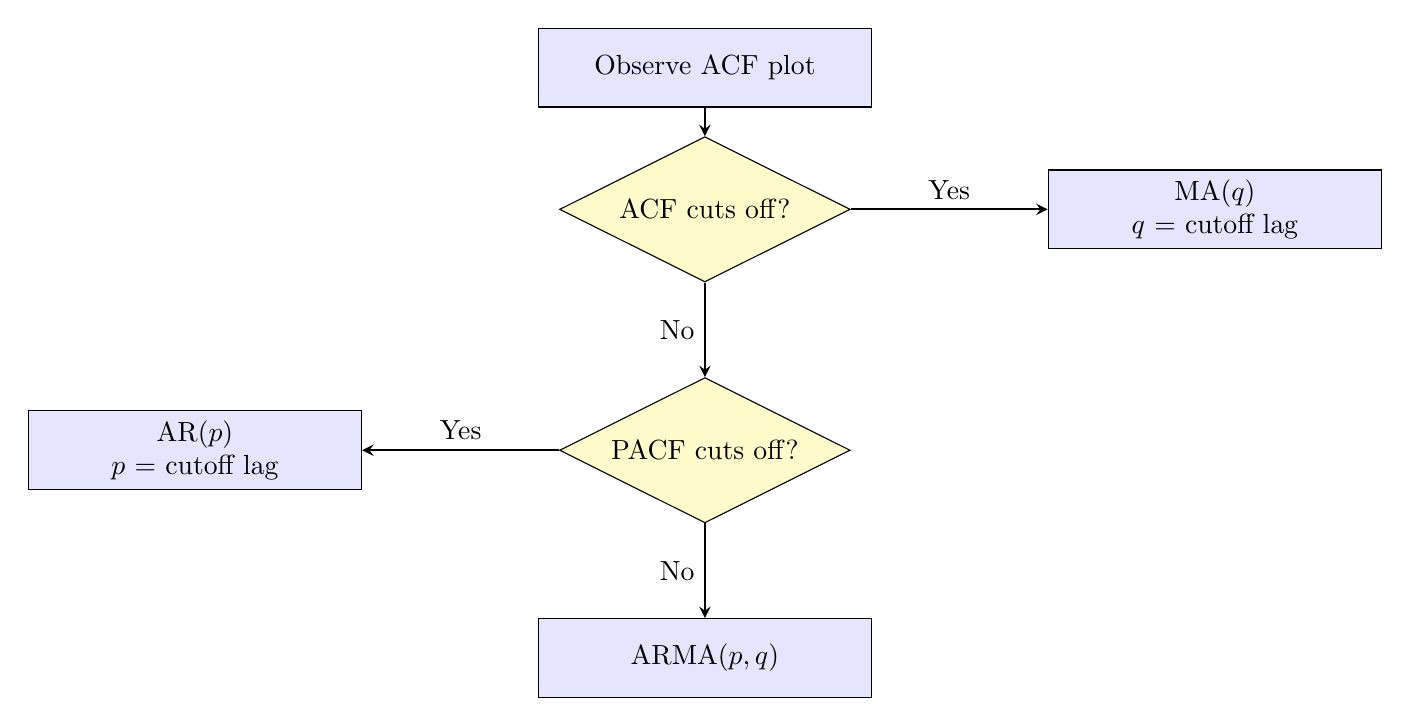
\begin{tikzpicture}[
    node distance=1.8cm,
    box/.style={rectangle, draw, fill=blue!10, text width=4cm, minimum height=1cm, align=center},
    decision/.style={diamond, draw, fill=yellow!20, text width=2.5cm, minimum height=1cm, align=center, aspect=2},
    arrow/.style={->, >=stealth, thick}
]
\node[box] (start) {Observe ACF plot};
\node[decision, below of=start] (acfcut) {ACF cuts off?};
\node[box, right=2.5cm of acfcut] (ma) {MA($q$)\\$q$ = cutoff lag};
\node[decision, below=1.2cm of acfcut] (pacfcut) {PACF cuts off?};
\node[box, left=2.5cm of pacfcut] (ar) {AR($p$)\\$p$ = cutoff lag};
\node[box, below=1.2cm of pacfcut] (arma) {ARMA($p,q$)};

\draw[arrow] (start) -- (acfcut);
\draw[arrow] (acfcut) -- node[above] {Yes} (ma);
\draw[arrow] (acfcut) -- node[left] {No} (pacfcut);
\draw[arrow] (pacfcut) -- node[above] {Yes} (ar);
\draw[arrow] (pacfcut) -- node[left] {No} (arma);
\end{tikzpicture}
\end{center}

\subsection{Seasonal Decomposition Diagram}

A time series $X_t$ can be decomposed into its constituent parts:

\begin{center}
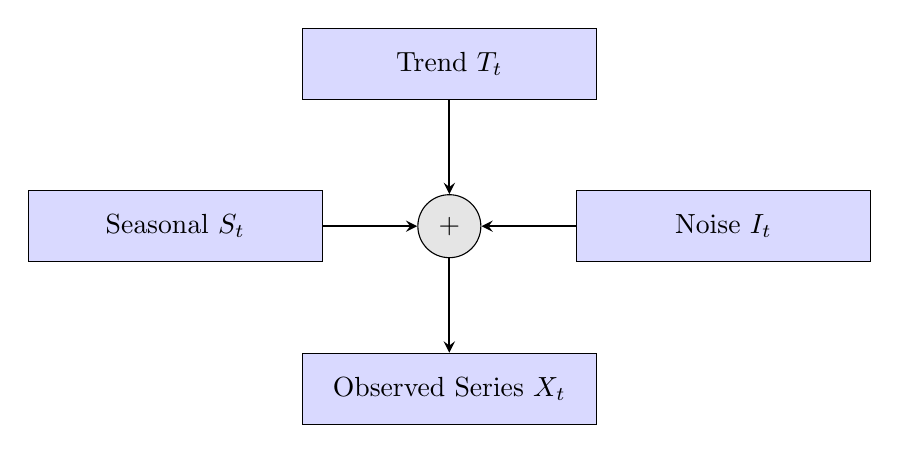
\begin{tikzpicture}[
    box/.style={rectangle, draw, fill=blue!15, text width=3.5cm, minimum height=0.9cm, align=center},
    sum/.style={circle, draw, fill=gray!20, minimum size=0.8cm, align=center},
    arrow/.style={->, >=stealth, thick}
]
\node[sum] (sum) at (0,0) {+};
\node[box, above=1.2cm of sum] (trend) {Trend $T_t$};
\node[box, left=1.2cm of sum] (seas) {Seasonal $S_t$};
\node[box, right=1.2cm of sum] (noise) {Noise $I_t$};
\node[box, below=1.2cm of sum] (series) {Observed Series $X_t$};

\draw[arrow] (trend) -- (sum);
\draw[arrow] (seas) -- (sum);
\draw[arrow] (noise) -- (sum);
\draw[arrow] (sum) -- (series);
\end{tikzpicture}
\end{center}

For the multiplicative model: $X_t = T_t \times S_t \times I_t$, the diagram would show multiplication ($\times$) instead of addition.

\subsection{AR(1) Stationarity Behavior Diagram}

\begin{center}
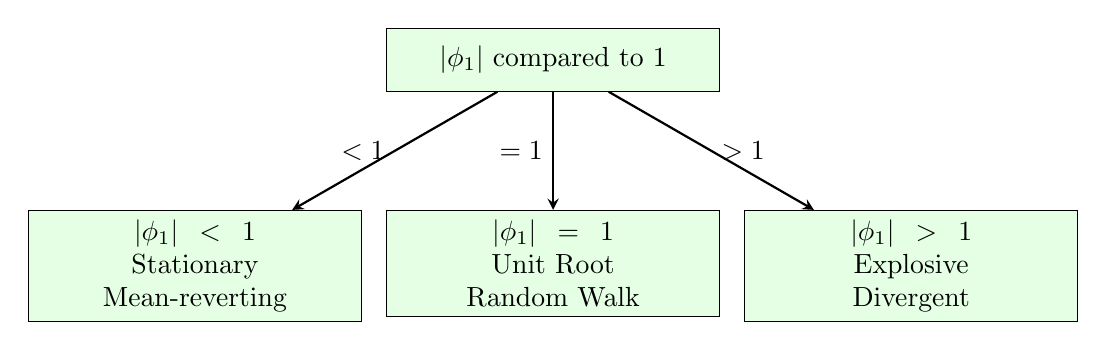
\begin{tikzpicture}[
    node distance=1.5cm,
    box/.style={rectangle, draw, fill=green!10, text width=4cm, minimum height=0.8cm, align=center},
    arrow/.style={->, >=stealth, thick}
]
\node[box] (phi) {$|\phi_1|$ compared to 1};
\node[box, below left=1.5cm and 0.3cm of phi] (lt) {$|\phi_1| < 1$\\Stationary\\Mean-reverting};
\node[box, below=1.5cm of phi] (eq) {$|\phi_1| = 1$\\Unit Root\\Random Walk};
\node[box, below right=1.5cm and 0.3cm of phi] (gt) {$|\phi_1| > 1$\\Explosive\\Divergent};

\draw[arrow] (phi) -- node[left] {$<1$} (lt);
\draw[arrow] (phi) -- node[left] {$=1$} (eq);
\draw[arrow] (phi) -- node[right] {$>1$} (gt);
\end{tikzpicture}
\end{center}

\section{Model Identification Summary: ACF and PACF Rules}

\begin{table}[H]
\centering
\begin{tabular}{|l|l|l|l|}
\hline
\textbf{Model} & \textbf{ACF Behavior} & \textbf{PACF Behavior} & \textbf{Rule} \\
\hline
AR($p$) & Tails off gradually & Cuts off after lag $p$ & If PACF cuts off at lag $p$, choose AR($p$) \\
MA($q$) & Cuts off after lag $q$ & Tails off gradually & If ACF cuts off at lag $q$, choose MA($q$) \\
ARMA($p,q$) & Tails off gradually & Tails off gradually & If both tail off, consider ARMA \\
White Noise & No significant spikes & No significant spikes & No AR or MA structure \\
\hline
\end{tabular}
\caption{ACF/PACF Identification Rules}
\end{table}

\textbf{Cut Off}: Becomes insignificant after a certain lag. Visual: significant spikes up to lag $k$, then zero.

\textbf{Tail Off}: Decreases gradually over many lags. Visual: slowly declining spikes.

\textbf{Exam Strategy}: Always examine the ACF first. If it cuts off, you have an MA. If it tails off, examine the PACF. If PACF cuts off, you have an AR. If both tail off, you have ARMA. For seasonal data, look for spikes at seasonal lags (e.g., lag 12 for monthly data) in addition to the non-seasonal pattern.

\begin{tcolorbox}[colback=green!5!white,colframe=green!75!black,title=\textbf{Worked Example 20: Seasonal Indices Calculation}]
\textbf{Given}: Quarterly sales (Rs lakhs):\\
2018: Q1=120, Q2=110, Q3=100, Q4=130\\
2019: Q1=125, Q2=115, Q3=105, Q4=135\\
2020: Q1=130, Q2=118, Q3=108, Q4=140\\
2021: Q1=135, Q2=120, Q3=112, Q4=145

\textbf{Find}: (a) Quarterly averages, (b) Grand average, (c) Seasonal indices, (d) Peak quarter, (e) Comment on seasonal variation.

\textbf{Solution}:
\begin{itemize}
    \item Q1 avg = $(120+125+130+135)/4 = 127.5$
    \item Q2 avg = $(110+115+118+120)/4 = 115.75$
    \item Q3 avg = $(100+105+108+112)/4 = 106.25$
    \item Q4 avg = $(130+135+140+145)/4 = 137.5$
    \item Grand avg = $(127.5+115.75+106.25+137.5)/4 = 486.75/4 = 121.6875$
    \item Q1 index = $127.5/121.6875 \times 100 \approx 104.77$
    \item Q2 index = $115.75/121.6875 \times 100 \approx 95.12$
    \item Q3 index = $106.25/121.6875 \times 100 \approx 87.31$
    \item Q4 index = $137.5/121.6875 \times 100 \approx 112.99$
\end{itemize}
\textbf{Peak season}: Q4 (112.99). \textbf{Low season}: Q3 (87.31). Sales are highest in Q4 (likely holiday season) and lowest in Q3. Q1 and Q2 are near average. The seasonal pattern is consistent across all four years, indicating stable seasonality.
\end{tcolorbox}

\begin{tcolorbox}[colback=green!5!white,colframe=green!75!black,title=\textbf{Worked Example 21: Seasonal Indices (5-Year Data)}]
\textbf{Given}: Year Q1 Q2 Q3 Q4: 2012:85,78,74,88; 2013:90,84,82,86; 2014:88,80,76,92; 2015:92,86,84,90; 2016:94,88,86,96.

\textbf{Find}: Seasonal indices and interpret.

\textbf{Solution}:
\begin{itemize}
    \item Q1 avg = $(85+90+88+92+94)/5 = 89.8$
    \item Q2 avg = $(78+84+80+86+88)/5 = 83.2$
    \item Q3 avg = $(74+82+76+84+86)/5 = 80.4$
    \item Q4 avg = $(88+86+92+90+96)/5 = 90.4$
    \item Grand avg = $(89.8+83.2+80.4+90.4)/4 = 343.8/4 = 85.95$
    \item Q1 index = $89.8/85.95 \times 100 \approx 104.48$
    \item Q2 index = $83.2/85.95 \times 100 \approx 96.80$
    \item Q3 index = $80.4/85.95 \times 100 \approx 93.54$
    \item Q4 index = $90.4/85.95 \times 100 \approx 105.18$
\end{itemize}
\textbf{Highest}: Q4 (105.18). \textbf{Lowest}: Q3 (93.54). The seasonal pattern shows Q4 as the peak quarter and Q3 as the trough, with Q1 slightly above average and Q2 slightly below. This is a classic seasonal pattern with stable amplitude across the five-year period.
\end{tcolorbox}

\end{document}
